\textbf{Метрики качества в задачах классификации}
\\
\textbf{1. Accuracy}\\
Accuracy - доля правильных ответов при классификации.
$$accuracy =\frac{true \ answers}{all \  answers} = \frac{T}{T + F}$$
\\
Accuracy бесполезна в задачах с неравными классами
\\

\textbf{Пример}
 Допустим, мы хотим оценить работу спам-фильтра почты. У нас есть 100 не-спам писем, 90 из которых наш
классификатор определил верно (True Negative = 90, False Positive = 10), и 10 спам-писем, 5 из которых классификатор
также определил верно (True Positive = 5, False Negative = 5). Тогда: accuracy =
$\frac{5+90}{5+90+10+5}$ = 86.4.
Однако если мы просто будем предсказывать все письма как не-спам, то получим более высокую accuracy: $\frac{0+100}{0+100+0+10}$ =
90.9
\\
\\
\textbf{2. Balanced accuracy} \\
Также есть ещё balanced accuracy. Когда мы знаем, что нам важны все классы, но мы знаем, что у одного
класса маленький размер. В таком случае мы можем сбалансировать и посчитать accuracy для каждого класса,
и уже полученные accuracy (их будет столько сколько классов) усреднить между собой. Но в реальной жизни
такая метрика оказывается довольно бесполезной, так как в такой агрегации нужно смотреть ещё на дисперсию, потому что повышая среднее, можно повысить еще и дисперсию (то есть у кого-то густо, у кого-то пусто).
Проблему дисбаланса классов такая метрика решает не очень хорошо.
$$balanced \ accuracy = \frac{1}{\#classes} \sum\limits_{\#classes} accuracy_i$$
\\
\\
 \textbf{4. Precision}\\
Precision - точность (классификация на 2 класса).(количество сбитых самолётов / общее количество выстрелов).
Количество правильных положительных ответов / общее количество положительных ответов.
\\
\begin{itemize}
    \item TP - истинно положительные
    \item FP - ложно положительные
    \item FN - ложно отрицательные
    \item TN - истинно отрицательные
\end{itemize}
\begin{center}
    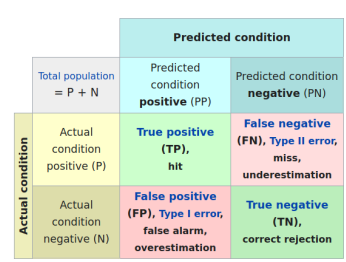
\includegraphics[]{2_1.PNG}
\end{center}
$$precision = \frac{TP}{TP+FP}$$
\\
\\
  \textbf{5. Recall}
\\
Recall - полнота. (количество сбитых самолётов / общее количество самолётов). Количество правильных положительных ответов / каким должно было быть количество положительных ответов.
$$recall =\frac{TP}{TP + FN}$$

Precision и recall не зависят, в отличие от accuracy, от соотношения классов и потому применимы в условиях несбалансированных выборок
\\
\\
\textbf{6. F-score}
\\
У нас есть две принципиально разных метрики - precision и recall, мы хотим минимизировать и ошибку 1 рода,
и ошибку 2 рода. Поэтому нам придется рассматривать то одну, то другую, как-то по очереди минимизировать,
это неудобно рассматривать две метрики одновременно. Соединим в себе две метрики, и будем брать минимум из них. Чуть-чуть подняв recall, мы чуть-чуть поднимаем precision. Такая метрика не дифференцируема
\begin{center}
    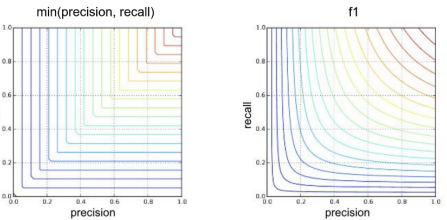
\includegraphics[]{2_2.PNG}
\end{center}
поэтому нам нужна более гладкая функция. Так появилась F1-score - гармоническое среднее между precision
и recall. Линии уровня имеют разный цвет, цветом отмечены различные значения f1-score. В правом верхнем
углу - идеальная ситуация.
$$F1 = 2\frac{1}{\frac{1}{precision}  + \frac{1}{recall}} = \frac{2 \cdot precision \cdot recall}{precision + recall}$$
\\
Как сделать так, чтобы важность precision и recall можно было пофиксить?
Например, вы решаете задачу машинного обучения в медицине, и вы хотите выделить людей, которые имеют
страшную болезнь. Вам выгоднее с точки зрения человеческих жизней, пресдказать лучше ложно человеку, что
он болен, чем пропустить человека и сказать больному, что он здоров. Таким образом recall для нас становится
важнее в этом примере.
Чтобы использовать F-score надо сдвинуть баланс, чтобы этот баланс соблюсти, у нас появляется параметр $\beta$.
$$F_{\beta} = (1 + \beta^2)\frac{  precision \cdot recall}{\beta^2 precision + recall}$$
\\
Член $1 + \beta^2$ нам нужен для нормировки, чтобы метрика оставалась между 0 и 1. Чтобы у нас был важнее
recall мы делаем $\beta < 1$ в знаменателе. В числителе обе метрики равнозначны.
\\
\\
\textbf{7.  ROC-AUC}\\
Если алгоритм бинарной классификации выдает не 0 и 1, а «вероятность 1», то чтобы дать конкретные ответы,
нужно выбрать порог. Чтобы оценивать алгоритм независимо от этого порога есть roc-auc. В нем перебирается этот
порог, и для каждого порога на графике откладываются точки (FPR, TPR). Получится ROC-кривая. Теперь чтобы
получить число, считается площадь под графиком AUC (area under ROC curve).
ROC-кривая - зависимость TPR (True Positive Rate) от FPR (False Positive Rate).
$$TPR = \frac{TP}{TP + FN}$$
$$FPR = \frac{FP}{FP + TN}$$
\\

\begin{center}
    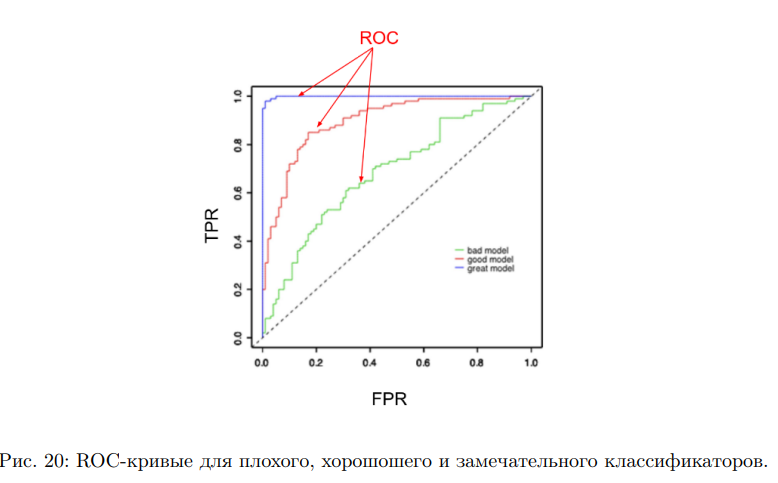
\includegraphics[]{2_4.PNG}
\end{center}
\\
\\
Главные свойства ROC кривой:
\begin{enumerate}
    
\item Baseline ялвяется случайным предсказанием, и лежит на линии y = x (диагонали на графике).
\item  Нормальный классификатор, который предсказывает что-то разумное, будет выше диагонали. Понятно,
что любой классификатор хороший, лучше чем случайное угадывание.
\item  Если предсказание лежит ниже baseline, то надо просто поменять знак, и тогда получится хороший
классификатор, кривая отразится относительно y = x.

\item Если график ROC одного классификатора строго выше (во всех точках) графика другого классификатора, то тот классификатор, который выше - лучше.
\item
Количество отсечек (ступенек) на кривой равно количеству объектов (не больше его). Если сетка установлена чаще, чем количество объектов, вы не получите ничего интересного
\end{enumerate}
\\
\textbf{Площадь под кривой ROC.} \\
Всё согласуется с тем, что мы постулировали, что чем выше кривая ROC, тем
лучше классификатор - площадь под кривой тоже будет больше. Тогда сложную кривую мы сведем к 1 числу.
По этому числу уже можно ранжировать модели между собой.
\begin{enumerate}
    \item Лежит в промежутке [0,1], но эффективно в [0.5,1], т.к. baseline имеет ROC-AUC = 0.5.
    \item Из того, что кривая лежит в каждой точке выше другой кривой, следует, что ROC-AUC у неё выше.
\end{enumerate}
Но наоборот не следует! Бывают случаи, когда один классификатор лучше в одной области, а другой в
другой области, а ROC-AUC у них равны.
\\
\\
\textbf{8.} \textbf{Мультиклассовые метрики}\\
Все предыдущие метрики были введены для бинарной классификации, чтобы перейти к метрикам мультиклассовой классификации, требуется взять среднее в каком-то смысле от метрик для всех бинарных классификаторов в мультиклассовой задаче. Буква S - сэмпл, то есть это вся выборка, а буква L - классы. В таблице показаны варианты мультиклассовых метрик из библиотеки sklearn.
\begin{center}
    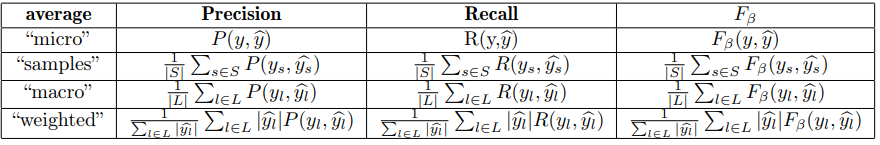
\includegraphics[]{2_5.PNG}
\end{center}


